\section{État actuel du projet et prévision pour la prochaine soutenance}
        
        Voici un tableau d'avancement des tâches réalisé et de nos prévisions pour la dernière soutenance : \\ \\
    
        {\normalsize
    	\begin{tabular}{|p{7cm}|p{2.4cm}|p{2.4cm}|}
    		\hline
    		Tâches & Actuellement & Soutenance \no 3 \\
    		\hline
    		Système de fichier & 100\% & 100\% \\
    		\hline
    		Sauvegarde & 50\% & 100\% \\
    		\hline
    		Compression & 50\% & 100\% \\
    		\hline
    		Chiffrement & 80\% & 100\% \\
    		\hline
    		Site web & 80\% & 100\% \\
    		\hline
    		Interface graphique & 25\% & 100\% \\
    		\hline
    	\end{tabular}
    	\label{répartition}}

\newpage

\section{Sauvegarde}
    
    \subsection{Système de fichier}
        \paragraph*{}
        Pour cette seconde soutenance, nous avons fini le système de fichiers. L'arbre représentant l'arborescence des fichiers ayant été créé pour la dernière soutenance, pour celle-ci, nous avons étoffé la structure de donnée qui contenait les données de chaque fichier. Ainsi, nous avons les structures metadata et metatree suivantes:
        
        \paragraph*{}
        \begin{lstlisting}[style=CStyle]
    struct meta_data
    {
        char *path;
        struct stat fs;
        off_t file_content
    }meta_data;
    
    struct meta_tree
    {
    struct meta_data *data;
    struct meta_tree *son;
    struct meta_tree *sibling;
    }meta_tree;
		\end{lstlisting}
        
        Ces deux structures de données permettent de représenter tous les fichiers a sauvegarder et ce sont ces structures de données qui sont sauvegardées avec le contenu de chaque fichier. L'élément file content ajoute représente l'offset du contenu du fichier lie au noeud représenté par la struct metatree. Il n'est défini et utile que lors de la restauration de sauvegarde et n'est jamais sauvegarde.
        Les fichiers de sauvegarde devront être tous places dans un même dossier pour chaque sauvegarde car il est nécessaire de toutes les avoir a portée en cas de restauration. Chaque fichier contenant une sauvegarde sera un .rdtgs qui sera notre type d'archive.
    \subsection{Sauvegarde}
        Pour cette soutenance 2, nous avons un début de sauvegarde. En effet, la sauvegarde initiale est créée cependant, toute la partie incrémentale n'est pas encore implémentée. Pour la sauvegarde normale, voici du pseudo code représentant l'algorithme de sauvegarde:
        
        \newpage
        \begin{lstlisting}[style=CStyle]
    sauvegarde(dossier_a_sauvegarde, chemin_de_la_sauvegarde)
    {
        créer le metatree du chemin dossier_a_sauvegarder
        pour chaque noeud de ce meta_tree:
            sauvegarder les données de la struct metadata associée sauf le file_content qui est inutile
            sauvegarder les liens du noeud (fils et ou frère)
            sauvegarder le contenu du fichier
        libérer le metatree
    }
		\end{lstlisting}
		Comme vous pouvez le voir, ce pseudo code a l'air simple. Cependant, de nombreux problèmes ont été rencontres pour l'implémenter. En effet, sauvegarder le contenu du fichier correctement s'est avéré plus complique que prévu car pour pouvoir le restaurer après il est nécessaire de sauvegarder sa taille, celle-ci étant calculee au fur et a mesure, il est nécessaire de sauvegarder la position dans le fichier de sauvegarde et de réserver de la place pour cette taille. Cela a pose quelques problèmes a cause d'une mauvaise compréhension du fonctionnement de certaines fonctions de la bibliothèque standard stdio telles que fseek, fwrite et fread (inversion de l'ordre de certains paramètres). 
    \subsection{Restauration}
        La restauration étant nécessaire pour tester la sauvegarde, elle a avance au même rythme que celle-ci. Ainsi, pour le moment, il est possible de restaurer une sauvegarde complète ou incomplète mais les sauvegardes incomplètes n'existant pas encore, cela n'est pas encore teste. Pour restaurer cette sauvegarde, nous suivons le pseudo code suivant:
        \begin{lstlisting}[style=CStyle]
        restauration(chemin_du_dossier_a_restaurer, chemin_de_la_sauvegarde)
        {
            charger l'arbre stocke dans la sauvegarde
            pour chaque noeud de l'arbre:
                si c'est un dossier(il a un fils)
                    recréer le dossier si il n'existe pas
                    appeler récursivement sur les fils
                sinon restaurer le contenu du fichier
            libérer l'arbre
        }
        charger_l'arbre_stocke_dans_une_sauvegarde(chemin_de_la_sauvegarde)
        {
            charger les méta données hors offset
            charger les liens
            récupérer l'offset et le stocker
            éviter le contenu du fichier sauvegarde
            en fonction des liens, appeler récursivement
        }        \end{lstlisting}
        
        
\newpage

\section{Compression}
    Avant de chiffrer les données et de réduire l'espace occupé, il est essentiel de les compresser auparavant. Comme exprimer dans le cahier des charges, ce sont les algorithmes de compression Huffman et LZ78 qui ont sélectionnés pour ce projet.
    
    Pour cette première soutenance, l'avancement est un peu plus faible que celui annoncé dans le cahier des charges. La raison ? Des lacunes. En effet, la vitesse de réalisation des algorithmes était beaucoup plus faible que prévu, dû un manque de compréhension sur les pointeurs du langage C.
    
    \subsection{Huffman}
        Pour cette soutenance, l'algorithme de compression de Huffman est opérationnel. En revanche, les contre-temps n'ont pas permis de mettre au point la décompression.
        La compression de Huffman se base sur la répétition des caractères pour la compression. Plus un caractère est présent dans la chaîne de départ plus il sera codé sur un nombre de bit réduit dans la chaîne compressée.
        En premier, nous construisons une liste avec tous les caractères présent et leur nombre d'apparition associé. Ce tableau doit être ensuite trié pour être utilisé. La liste est triée dans l'ordre décroissant.
        Avec la liste obtenue, nous construisons un arbre binaire où chaque feuille contient un caractère de la précédente liste. Les noeud interne ne contiennent pas de valeur utile. Dans la théorie ils contiennent $\epsilon$, dans notre projet, ils contiendront le caractère NULL. La construction de l'arbre se passe de la sorte (pour une chaîne contenant au moins trois caractères différents) : 
        \begin{enumerate}
            \item Les deux premiers éléments sont placés en feuille et sont fils d'un unique noeud père. Ce dernier devient le fils gauche du noeud racine de l'arbre final.
            \item Un noeud contenant $\epsilon$ est ajouté en fils droit de la racine. Et nous plaçons un pointeur sur ce dernier
            \item Les deux éléments suivant, s'ils existent sont ajoutés en fils et feuille d'un unique noeud père. Ce dernier devient le fils gauche du noeud pointé
            \item Un noeud contenant $\epsilon$ est ajouté en fils droit du noeud pointé. Le pointeur est déplacé sur son fils droit.
            \item Quand il n'y a plus d'élément, l'avant dernier fils droit de l'arbre final est remplacé par le fils gauche de ce dernier.
        \end{enumerate}
        Les étapes 3 et 4 sont répétées récursivement jusqu'à qu'il n'y ait plus d'élément dans la liste.
        Il reste à construire la table de codage qui donne la représentation binaire de chaque caractère de la chaîne. La méthode est simple : il suffit de faire un parcours profondeur de l'arbre en ajoutant en préfixe un 0 si on passe sur un fils gauche, ou un 1 si on passe sur un fils droit. Dès qu'on arrive sur une feuille on ajoute à la table de codage, le contenu de la chaîne préfixe et la valeur de la clé de la feuille.
        Il a été remarqué que nous pouvons utiliser la table de codage pour reconstruire l'arbre. Ainsi, nous la recyclons pour la compression de l'arbre de Huffman. Cette manipulation nous évite de refaire plusieurs parcours de l'arbre et d'allouer une autre liste, ce qui optimise significativement le temps et les ressources nécessaire au programme de compression.
        Pour encoder la chaîne en entrée, il nous suffit de remplacer tout les caractères par leur équivalent dans la table de codage. Elle sera alors en binaire; la dernière étape consiste à convertir le binaire en ASCII et passer d'une liste chaînée dynamique à une chaîne de caractère statique.
        Pour l'encodage de l'arbre, il suffit de convertir en binaire tous les caractères différents de 0 ou de 1 en binaire et reconvertir en ASCII l'ensemble.
        Pendant la conversion en binaire, la longueur des chaînes de caractères des données et/ou de l'arbre ne sont pas nécessairement un multiple de 8, c'est pourquoi il est nécessaire de rajouter des 0 pour compléter. Cette manipulation nous oblige a transmettre le nombre de bits rajouté pour l'alignement.
        
        Mais huffman n'est pas utilisé dans tous les cas. Lorsqu'il n'y a pas suffisamment de caractères différents présent dans la chaîne, un autre algorithme plus léger est appliqué à la place. Lorsque le nombre de caractères différents est inférieur ou égal à 4, on sait par avance le nombre de bits utilisé pour chaque caractère et que ce sera le même pour tous les caractères indépendamment de leur nombre d'occurrence dans la chaîne. 1 bit pour chaque caractère quand il y a un ou deux caractères différents; 2 bits pour chaque caractère quand il y a trois ou quatre caractères différents. Elle est dans le même état d'esprit que Huffman a l'exception près que l'on connaît par avance le nombre de bit de codage et donc il n'y a pas besoin de construire d'arbre, de table de codage : la chaîne finale est construite directement.
        
        Une fois les chaînes et/ou les arbres encodés, il faut encapsuler les données pour qu'elles puissent tenir dans une unique chaîne de caractère qui sera retournée par le programme. Il faut donc définir la position de chaque donnée dans la chaîne pour que la fonction de décompression puisse re-séparer les données et opérer à leur décompression. Le premier octet de la chaîne indique si c'est l'algorithme de Huffman (avec une valeur supérieur à 128) ou l'autre algorithme. Dans ce dernier cas, cet octet indique le nombre de caractères différent de la chaîne d'origine (1, 2, 3 ou 4). Ensuite en commun entre les deux algorithmes, le nombre de bits d'alignement. Puis sur cinq octets la longueur de la chaîne encodée. Pour l'instant, la longueur est en base 10, ce qui met un maximum de 9999 caractères compressés. Pour la troisième soutenance, les données concernant la longueur seront codés en base 256 ce qui offrera une limite théorique de $256^{5} - 1$. A partir de maintenant, les données diffèrent entre les deux algorithmes :\newpage
        \begin{itemize}
            \item \textbf{\underline{Algorithme de Huffman}}
                \begin{enumerate}
                    \item \textbf{Type d'algorithme employé} : Codé sur 1 octet, il confirme s'il s'agit d'Huffman ou de l'autre. Pour Huffman, cette valeur est supérieure à 128.
                    \item \textbf{Bits d'alignement} : Codé sur 1 octet, il indique le nombre de bits à ne pas prendre en compte à la fin de la chaîne encodée.
                    \item \textbf{Longueur de la chaîne encodée} : Codée sur 5 octets en base 10, elle offre une limite théorique de 9 999 caractères encodés maximum. Pour la dernière soutenance, elle sera encodée en base 256 ce qui montera la limite théorique à : $256^{5} - 1$.
                    \item \textbf{Chaîne encodée} : Codé sur autant d'octet que la longueur donnée précédemment. Elle contient toute les données de la chaîne.
                    \item \textbf{Bits d'alignement de l'arbre} : Codé sur 1 octet, il indique le nombre de bits à ne pas prendre en compte à la fin de l'arbre encodé.
                    \item \textbf{Longueur de l'arbre encodée} : Codée également sur 5 octets en base 10. Elle subira les mêmes modifications que sa collègue de data.
                    \item \textbf{Arbre encodé} : Codé sur autant d'octet donné par la précédente longueur. Il contient l'arbre de Huffman sous forme d'une chaîne de caractères.
                \end{enumerate}
            \item \textbf{\underline{Algorithmes petite différence}}
                \begin{enumerate}
                    \item \textbf{Type d'algorithme employé} : Codé sur 1 octet, il différencie une chaîne compressée par Huffman en étant inférieur à 128. Pour éviter de perdre un octet pour rien, il prend la valeur du nombre de caractère différent de la chaîne originel.
                    \item \textbf{Bits d'alignement} : Codé sur 1 octet, il donne le nombre de bit à ne pas prendre en compte à la fin de la chaîne encodée.
                    \item \textbf{Longueur de la chaîne encodée} : Codée sur 5 octets en base 10. Comme pour Huffman, ce choix offre une forte limitation sur la taille maximale de la chaîne brute encodée. Cependant, il a été montré que nous pouvions nous en passer. A la prochaine soutenance, nous ne trouverons plus cette information dans le fichier de sortie.
                    \item \textbf{Chaîne encodée} : Codé sur autant d'octet que la longueur donnée précédemment. Elle contient la chaîne originel compressée.
                    \item \textbf{Caractères disponibles} : Codé sur autant d'octet que la longueur donnée dans le premier octets, on y trouve les valeurs ASCII de tous les caractères différents présents dans la chaîne originel.
                \end{enumerate}
        \end{itemize}
        
        Une fonction chapeau a été rajouté pour ajouter une gestion minimale des fichiers en entrée et sortie du programme. Ce dernier prend en paramètre le chemin d'accès au fichier à compresser. Il récupère le contenu, le compresse, créer un fichier du même nom à côté du fichier d'entrée mais avec l'extension \textit{.huf} en plus si ce dernier n'existe pas. Puis écrit dans ce fichier le résultat de la compression. Pour cette soutenance, il affiche dans le terminal le ratio final et l'emplacement du fichier compressé.
        Le calcul du ratio en pourcentage est élémentaire :
        \[
            ratio = \frac{poids(fichier compressé)}{poids(fichier entrée)} * 100
        \]
        
        Pour la troisième soutenance, un deuxième algorithme de compression sera disponible : LZ78. Il s'agit d'un algorithme de compression par dictionnaire.
        En bonus pour la troisième soutenance, serait de faire un algorithme qui combine LZ78 et huffman pour implémenté un algorithme très utilisé dans le monde, le \textbf{deflate}. Il est notamment utilisé pour compressé au format ZIP.
        
    
\newpage

\section{Chiffrement}
    
        Pour cette soutenance, AES a été fixé et RSA a été optimisé pour pouvoir générer des clefs RSA de taille élevé.

        \subsection{Rotn}
        Nous avons tout d’abord implémenté l’algorithme Rotn.
        Cette algorithme de chiffrement par substitution utilise une clé qui est un simple entier.
        C’est une généralisation du Chiffre de César. \\
        Il consiste à remplacer systématiquement dans le message clair une lettre donnée (dans notre cas un code ascii) de l'alphabet par un signe donné en fonction de la clé. C’est donc une simple addition pour chaque charactère du code ascii du caractère avec la clé.
        Le déchiffrement est donc la différence du caractère encodé avec la clé. \\ \\

        \subsection{Vigenère}
            Le chiffre de Vigenère est un système de chiffrement par substitution, mais une même caractère du message clair peut, suivant sa position dans celui-ci, être remplacée par des lettres différentes en fonction de la clé qui, contrairement à un système de chiffrement tel que Rotn ou le chiffre de César, est d’une chaine de caractère. Cette méthode résiste ainsi à l'analyse de fréquences. Il suit le même fonctionnement que Rotn à la différence que l’on utilise les caractères de la clé pour chiffrer le message. \\
        
        \newpage

        \subsection{RSA}
        Nous avons aussi été implémenté l’algorithme de chiffrement asymétrique RSA. Pour la réalisation de cet algorithme, nous avons utilisé la bibliothèque (The GNU Multiple Precision Arithmetic Library \url{https://gmplib.org/}) pour éviter tous overflow dû au fonctionnement d’RSA. Cette bibliothèque nous met à disposition le type de donnes mpz\_t, qui nous permet de travailler avec de grands nombres sans craindre un overflow.
        Notre algorithme génère désormais la clé privée et la clé publique de facon aléatoire à partir d'un entier N qui est la taille de la clefs (par exemple, 2048 pour un clefs de 2048 bits). Cette algorithme génère donc 2 entiers premiers de taille $2^{N-1}$ bits P et Q. On a donc ensuite $N = P * Q$.
        Via le théorème de Bachet-Bézout, nous générons ensuite l'exposant de chiffrement E et l'exposant de déchiffrement D via l'algorithme d'Euclide étendu.

        \begin{lstlisting}[style=CStyle]
    struct RSA_publickey {
        mpz_t *n;
        mpz_t *e;
    } RSA_publickey;
    
    struct RSA_privatekey {
        mpz_t *n;
        mpz_t *d;
    } RSA_privatekey;
		\end{lstlisting}	
		
       \begin{lstlisting}[style=CStyle]
    struct RSA_publickey *RSA_gen_public_key(mpz_t p, mpz_t q);
    
    struct RSA_privatekey *RSA_gen_private_key(mpz_t p, mpz_t q, struct RSA_publickey *public);
		\end{lstlisting}s

        Pour chiffrer, nous avons juste besoin d’appeler la fonction RSA\_encode avec la clé publique et une chaine de caractère. Cette fonction nous retourne la chaine encodée sous la forme d’un tableau de mpz\_t et chiffre le texte via la formule C &\equiv ~ $M^{E}$ mod N.

        La fonction RSA\_decode permet de déchiffrer le tableau de mpz\_t avec la clé privée et nous retourne la chaine de caractère décodée et déchiffre le texte via la formule C &\equiv ~ $M^{D}$ mod N. \\


	\subsection{AES}
        AES est un algorithme de chiffrement symétrique par bloc de 16 caractères (sous la forme de matrice). Dans la version AES 128, que nous avons implémenté, il est constitué d’un algorithme d’expansion de la clé qui nous permet d’obtenir 10 autres clés devant être utilisé pour le chiffrement/déchiffrement et de 4 algorithmes (AddRoundKey, Subbytes, Shiftrows, Mixcolumns, KeyExpansion) utilisé dans l’algorithme de chiffrement (pour le déchiffrement, l’inverse de ces 4 algorithmes est utilisé).
        AES 128 ECB utilise donc ces différents algorithmes pendant les 10 tours nécessaires à son fonctionnement.
        L’algorithme de déchiffrement reprend le même principe.

        Nous avons donc créé une nouvelle structure AES\_matrix pour simplifier la création des algorithmes.

        \begin{lstlisting}[style=CStyle]
    struct AES_matrix {
        size_t rowsLenght;
        size_t colsLenght;
        uint8_t **data;
    } AES_matrix;
		\end{lstlisting}	

        AES 128 ECB est désormais opérationnel. Il fonctionne aussi bien pour chiffrer et déchiffrer des fichiers. \\

        Pour la prochaine soutenance, nous implémenterons le  cryptosystème d'ElGamal. \\
\newpage

\section{L'interface graphique}
    Un logiciel de sauvegarde peut être compliquer à utiliser pour l'utilisateur. C'est pour cela qu'une interface graphique est plus que nécessaire. \\
    Bien qu'elle ne doit pas être excessivement complète et qu'elle peut reste simple d'utilisation, l'interface devra tout de même fournir tous les outils nécessaire pour compresser et chiffrer les document désires. \\
    Les objectifs actuellement fixe pour une interface sont donc les suivant: Une interface simple et efficace réalisé grâce à la librairie GTK-3, donner accès a tous les outils nécessaire à l'utilisateur pour effectuer des sauvegardes, permettre à l'utilisateur de sélectionner les fichiers et document à compresser/chiffrer et créer une interface appréciable à regarder, pouvant informer l'avancement du programme après son exécution. \\
    
    L'interface actuelle est composé d'une simple fenêtre avec deux bouton qui ouvre deux nouvelles fenêtres, les autres boutons ne servent à rien, autre que d'afficher sur le terminal qu'ont à appuyer dessus. La création de cette interface fut possible à l'aide du logiciel Glade, permettant la construction d'un squelette pour une interface, par la suite relié à un code en C pour rendre le tout fonctionnelle. L'interface à été raffinée pour obtenir une interface présentable en soutenance, mais toujours non fonctionnel pour les boutons qui n'effectue qu'une fonction basique pour le moment. \\
    L'interface n'est pas au point pour être utilisé par un utilisateur lambda et la dernière étape à faire est d'adapter l'interface pour pouvoir être utilisé par n'importe qui. \\
    La version finale de l'interface devra proposé le choix entre sauvegarder ou restaurer un fichier, en proposant les options de compression et de chiffrement à l'utilisateur. 
    
	\begin{figure}[!h]
		\centering
		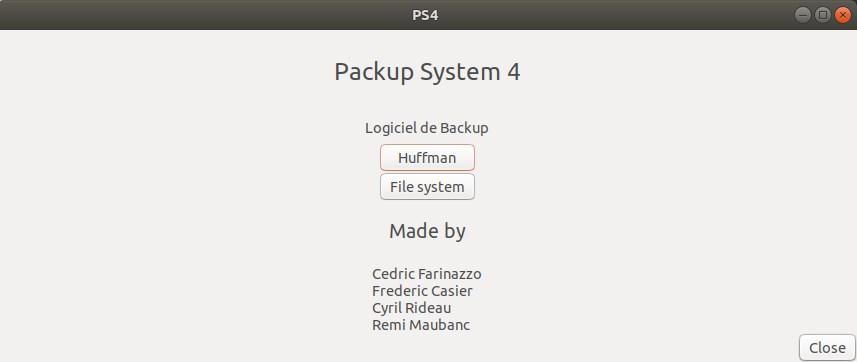
\includegraphics[width=13.1cm]{images/gui-screen.png}
		\caption{Interface actuel}
		\label{Interface actuel}
	\end{figure}
	
	
    
\newpage

\section{Site web}

    Le site web est disponible à l'adresse suivante: \url{https://packup.hyperion.tf/}. \\
    Il est actuellement hébergé sur un VPS\footnote{VPS (Virtual Private Server) = Serveur privé virtuel} d'OVH déjà utilisé par Hyperion pour herbergé plusieurs sites web. Ce serveur était idéal car il possède une configuration opérationnelle. Notre choix pour les parties de back-end et de front-end ont été très largement influencé par les infrastructure web déjà en place. Ainsi, nous avons choisit le framework Django \url{https://www.djangoproject.com/} pour le site web qui fait appel au serveur d'application uwsgi et au reverse proxy nginx.
    Pour le style et l'affichage, nous utilisons le framework Materialize (\url{https://materializecss.com/}) afin de vous présenter un site web clair et responsive.

    Notre cahier des charges et les rapports de soutenance sont aussi disponibles sur ce dernier.
    
    Comme prévu, pour cette soutenance, nous avons ajouté le système d'authentification.
    L'utilisateur peut donc créer un compte, se connecter, modifier ces informations.
    
    Pour la dernière soutenance, nous permettrons à l'utilisateur d'envoyer une archive générer par notre programme sur le site web.
    \begin{figure}[!h]
		\centering
		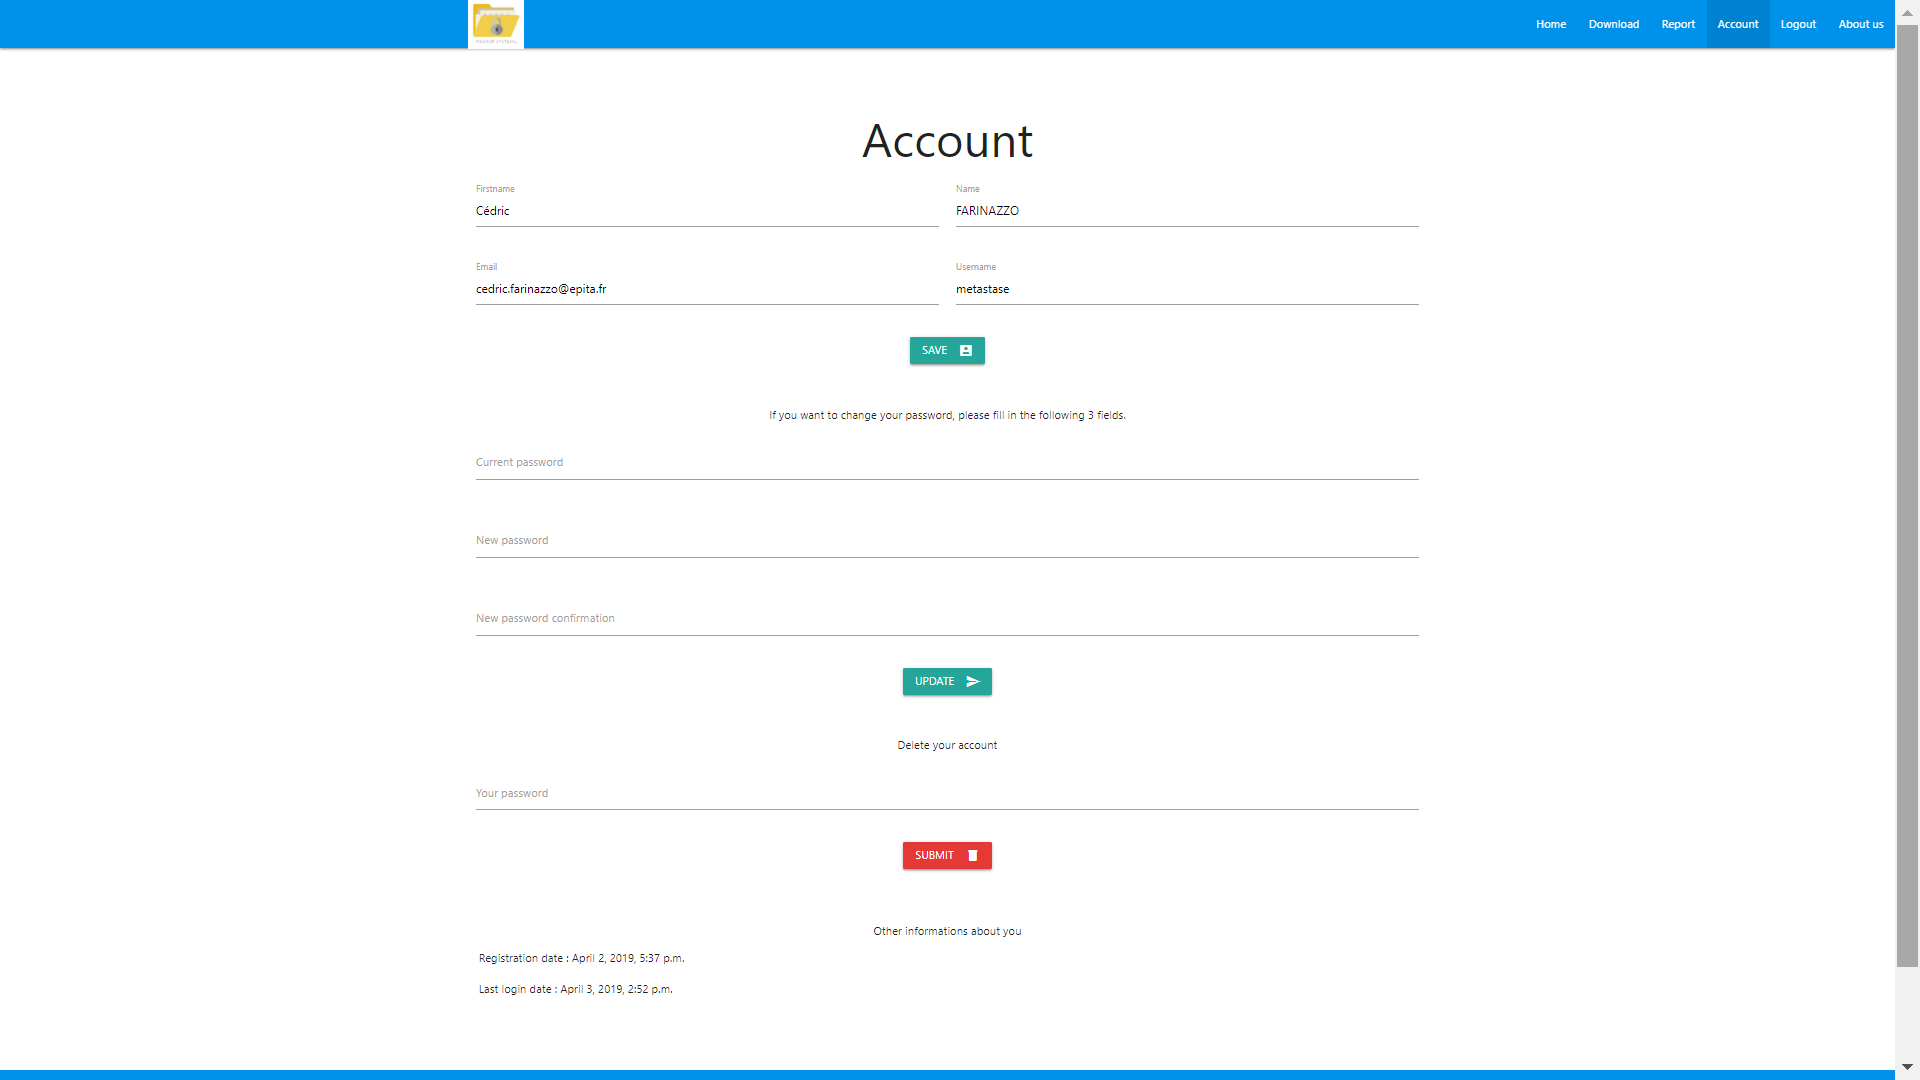
\includegraphics[width=8cm]{images/website-account.png}
		\caption{Page permettant de gérer les informations du compte}
		\label{Site web actuel}
	\end{figure}
    
    \begin{figure}[!h]
		\centering
		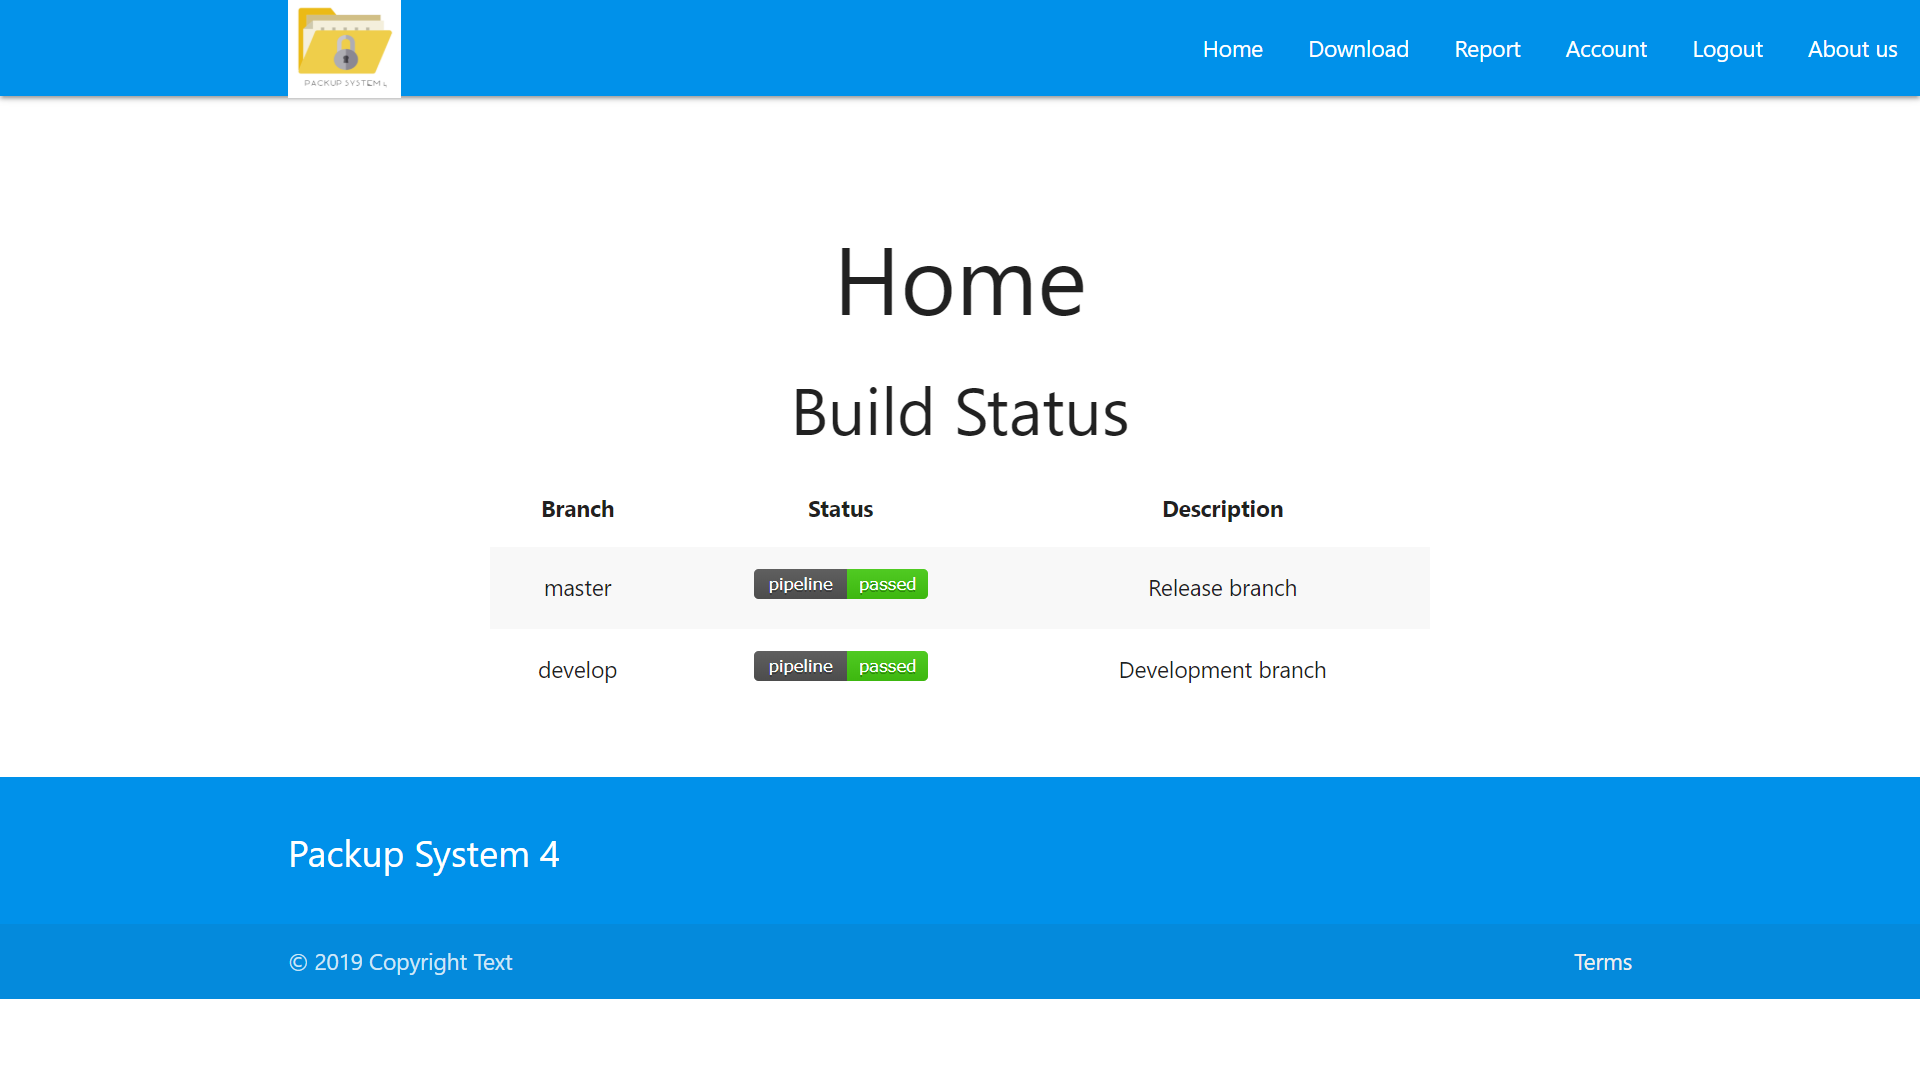
\includegraphics[width=8cm]{images/website.png}
		\caption{Site web actuel}
		\label{Site web actuel}
	\end{figure}

\newpage

\section{Avancement prévu pour les prochaines soutenances}
        
        Voici un tableau d'avancement des tâches prévu pour les prochaines soutenances : \\ \\
    
        {\normalsize
    	\begin{tabular}{|p{7.6cm}|p{1.8cm}|p{1.8cm}|p{1.8cm}|}
    		\hline
    		Tâches & \multicolumn{3}{|c|}{Soutenance} \\ 
    		\cline{2-4}
    			& \no 1 & \no 2 & \no 3 \\
    		\hline
    		Système de fichier & 75\% & 100\% & 100\% \\
    		\hline
    		Sauvegarde & 50\% & 75\% & 100\% \\
    		\hline
    		Compression & 30\% & 60\% & 100\% \\
    		\hline
    		Chiffrement & 30\% & 80\% & 100\% \\
    		\hline
    		Site web & 50\% & 80\% & 100\% \\
    		\hline
    		Interface graphique & 25\% & 60\% & 100\% \\
    		\hline
    	\end{tabular}
    	\label{répartition}}